\chapter{Les boucles}
\label{les-boucles}

Dans ce chapitre, nous allons aborder les \textbf{boucles}.
Une boucle est un moyen de répéter des instructions
suivant le résultat d'une condition. Ces structures, dîtes
\textbf{itératives}, que nous allons voir dans ce chapitre sont les
suivantes.

\begin{table}
\centering
\rowcolors{1}{gris-clair-tab}{}
\begin{tabular}{|p{3cm}|p{12cm}|}\hline
\rowcolor{gris-tab-entete}\textbf{\makecell{Structure \\itérative}} & \textbf{\makecell{Action}}\tabularnewline\hline
\textbf{\emph{while\ldots{}}} & répète une suite d'instructions tant qu'une condition est respectée.\tabularnewline\hline
\textbf{\emph{do\ldots{} while\ldots{}}} & répète une suite d'instructions tant qu'une condition est respectée. Le groupe d'instructions est exécuté au moins une fois.\tabularnewline\hline
\textbf{\emph{for\ldots{}}} &  répète un nombre fixé de fois une suite d'instructions.\tabularnewline\hline
\end{tabular}
\end{table}

\section{La boucle while}
\label{la-boucle-while}

La première des boucles que nous allons étudier est la boucle
\mybox{while} (qui signifie « tant que »). Celle-ci permet de répéter
un bloc d'instructions tant qu'une condition est remplie.

\begin{figure}[htbp]
\centering
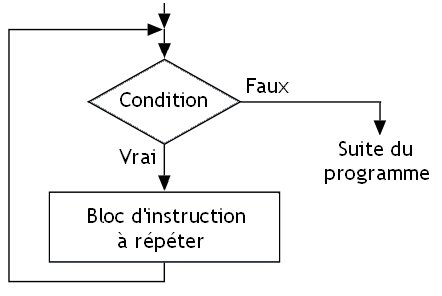
\includegraphics[scale=0.4]{images/structure-while.jpg}
\caption{Structure While}
\end{figure}

\subsection{Syntaxe}
\label{syntaxe-1}

La syntaxe de notre boucle \mybox{while} est assez simple.

\begin{C}
while (/* Condition */)
{
    /* Bloc d'instructions à répéter */ 
}
\end{C}

\subsubsection{Exemple}
\label{exemple-5}

\begin{C}
#include <stdio.h>


int main(void)
{
    int i = 0;

    while (i < 5)
    {
        printf("La variable i vaut %d\n", i);
        i++;
    }

    return 0;
}
\end{C}

\begin{C}
La variable i vaut 0
La variable i vaut 1
La variable i vaut 2
La variable i vaut 3
La variable i vaut 4
\end{C}

Le fonctionnement est simple à comprendre :

\begin{itemize}
\item
  Au départ, notre variable \mybox{i} vaut zéro. Étant donné que zéro
  est bien inférieur à cinq, la condition est vraie, le corps de la
  boucle est donc exécuté.
\item
  La valeur de \mybox{i} est affichée.
\item
  \mybox{i} est augmentée d'une unité et vaut désormais un.
\item
  La condition de la boucle est de nouveau vérifiée.
\end{itemize}

Ces étapes vont ainsi se répéter pour les valeurs un, deux, trois et
quatre. Quand la variable \mybox{i} vaudra cinq, la condition sera
fausse, et l'instruction \mybox{while} sera alors passée.

\begin{infobox}
  Dans cet exemple, nous utilisons une
variable nommée \mybox{i}. Ce nom lui vient d'une contraction du mot
anglais \emph{iterator} qui signifie que cette variable sert à
l'itération (la répétition) du corps de la boucle. Ce nom est tellement
court et explicite qu'il est pour ainsi dire devenu une convention de
nommage en C.
\end{infobox}

\subsection{Exercice}
\label{exercice-3}

Essayez de réaliser un programme qui détermine si un nombre entré par
l'utilisateur est premier. Pour rappel, un nombre est dit premier s'il
n'est divisible que par un et par lui-même. Notez que si un nombre \(x\)
est divisible par \(y\) alors le résultat de l'opération
\mybox{x\ \%\ y} est nul.

\subsubsection{Indice}
\label{indice-1}

\begin{secretbox}
 Pour savoir si un nombre est premier, il
va vous falloir vérifier si celui-ci est uniquement divisible par un et
lui-même. Dit autrement, vous allez devoir contrôler qu'aucun nombre
compris entre 1 et le nombre entré (tout deux exclus) n'est un diviseur
de ce dernier. Pour parcourir ces différentes possibilités, une boucle
va vous être nécessaire.
\end{secretbox}


\subsubsection{Correction}
\label{correction-4}

\begin{C}
 #include <stdio.h>


int main(void)
{
   int nombre;
   int i = 2;

   printf("Entrez un nombre : ");
   scanf("%d", &nombre);

   while ((i < nombre) && (nombre % i != 0))
   {
       ++i;
   }

   if (i == nombre)
   {
       printf("%d est un nombre premier\n", nombre);
   }
   else
   {
       printf("%d n'est pas un nombre premier\n", nombre);
   }

   return 0;
}
\end{C}

\section{La boucle do-while}
\label{la-boucle-do-while}

La boucle \mybox{do\ while} fonctionne comme la boucle \mybox{while},
à un petit détail près : elle s'exécutera toujours au moins une fois,
alors qu'une boucle \mybox{while} peut ne pas s'exécuter si la
condition est fausse dès le départ.

\begin{figure}[htbp]
\centering
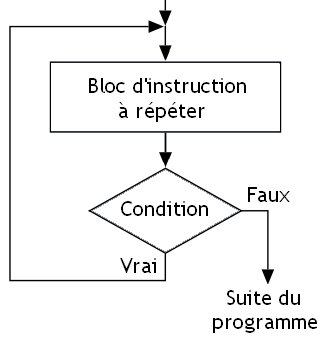
\includegraphics[scale=0.4]{images/instruction_do_while.jpg}
\caption{Instruction do\ldots{} while\ldots{}}
\end{figure}

\subsection{Syntaxe}
\label{syntaxe-2}

À la différence de la boucle \mybox{while}, la condition est placée à
la fin du bloc d'instruction à répéter, ce qui explique pourquoi
celui-ci est toujours exécuté au moins une fois. Remarquez également la
présence d'un point-virgule à la fin de l'instruction qui est
obligatoire.

\begin{C}
do
{
    /* Bloc d'instructions à répéter */
} while (/* Condition */);
\end{C}

\subsection{Exemple 1}
\label{exemple-6}

Voici le même code que celui présenté avec l'instruction \mybox{while}.

\begin{C}
#include <stdio.h>


int main(void)
{
    int i = 0;

    do
    {
        printf("La variable i vaut %d\n", i);
        ++i;
    } while (i < 5);

    return 0;
}
\end{C}

\begin{C}
La variable i vaut 0
La variable i vaut 1
La variable i vaut 2
La variable i vaut 3
La variable i vaut 4
\end{C}

\subsection{Exemple 2}
\label{exemple-7}

Comme nous vous l'avons dit plus haut, une boucle \mybox{do\ while}
s'éxecute au moins une fois.

\begin{C}
#include <stdio.h>


int main(void)
{    
    do
        printf("Boucle do-while\n");
    while (0);

    return 0;
}
\end{C}

\begin{C}
Boucle do-while
\end{C}

Comme vous le voyez, malgré que la condition est fausse (pour rappel,
une valeur nulle correspond à une valeur fausse), le corps de la boucle
est exécuté une fois puisque la condition n'est évaluée qu'\emph{après}
que le bloc d'instructions ait été parcouru.

\section{La boucle for}
\label{la-boucle-for}


\subsection{Syntaxe}
\label{syntaxe-3}

\begin{C}
for (/* Expression 1 */ ; /* Condition */ ; /* Expression 2 */)
{
    /* Instructions à répéter */
}
\end{C}

Une boucle \mybox{for} se décompose en trois parties :

\begin{itemize}
\item
  une expression, qui sera le plus souvent l'initialisation d'une
  variable ;
\item
  une condition ;
\item
  une seconde expression, qui consistera le plus souvent en
  l'incrémentation d'une variable.
\end{itemize}

Techniquement, une boucle \mybox{for} revient en fait à écrire ceci.

\begin{C}
/* Expression 1 */

while (/* Condition */)
{
    /* Bloc d'instructions à répéter */
    /* Expression 2 */
}
\end{C}

\subsection{Exemple}
\label{exemple-8}

Le fonctionnement de cette boucle est plus simple à appréhender à l'aide
d'un exemple.

\begin{C}
#include <stdio.h>


int main(void)
{
    int i;

    for (i = 0 ; i < 5 ; ++i)
        printf("la variable i vaut %d\n", i);

    return 0;
}
\end{C}

\begin{C}
variable vaut 0
variable vaut 1
variable vaut 2
variable vaut 3
variable vaut 4
\end{C}

Ce qui, comme dit précédemment, revient exactement à écrire cela.

\begin{C}
#include <stdio.h>


int main(void)
{
    int i;

    i = 0;

    while (i < 5)
    {
        printf("la variable i vaut %d\n", i);
        ++i;
    }

    return 0;
}
\end{C}

\begin{attentionbox}
  Notez bien que la première expression,
\mybox{i\ =\ 0}, est située \emph{en dehors} du corps de la boucle.
Elle n'est donc pas évaluée à chaque tour.
\end{attentionbox}

\subsubsection{Exercice}
\label{exercice-4}

Essayez de réaliser un programme qui calcule la somme de tous les
nombres compris entre un et \(n\) (\(n\) étant déterminé par vos soins).
Autrement dit, pour un nombre \(n\) donné, vous allez devoir calculer
\(1 + 2 + 3 + ... + (n-2) + (n-1) + n\).

\begin{C}
 #include <stdio.h>


int main (void)
{
    const unsigned int n = 250;
    unsigned int somme = 0;
    unsigned int i;

    for (i = 1; i <= n; ++i)
        somme += i;

    printf ("Somme de 1 à %u : %u\n", n, somme);
    return 0;
}
\end{C}

\begin{infobox}
 Notez qu'il est possible de réaliser
cet exercice sans boucle en calculant : \(\frac {N \times (N+1)} {2}\).
\end{infobox}

\subsection{Plusieurs compteurs}
\label{plusieurs-compteurs}

Notez que le nombre de compteurs ou de conditions n'est pas limité,
comme le démontre le code suivant.

\begin{C}
for (i = 0, j = 2 ; i < 10 && j < 12; i++, j += 2)
\end{C}

Ici, nous définissons deux compteurs \mybox{i} et \mybox{j}
initialisés respectivement à zéro et deux. Le contenu de la boucle est
exécuté tant que \mybox{i} est inférieur à dix et que \mybox{j} est
inférieur à douze, \mybox{i} étant augmentée de une unité et \mybox{j}
de deux unités à chaque tour de boucle. Le code est encore assez
lisible, cependant la modération est de mise, un trop grand nombre de
paramètres rendant la boucle \mybox{for} illisible.

\section{Imbrications}
\label{imbrications}

Il est parfaitement possible d'\textbf{imbriquer} une ou plusieurs
boucles en plaçant une boucle dans le corps d'une autre boucle.

\begin{C}
int i;
int j;

for (i = 0 ; i < 1000 ; ++i)
{
    for (j = i ; j < 1000 ; ++j)
    {
          /*  Code  */
    }
}
\end{C}

Cela peut servir par exemple pour déterminer la liste des nombres dont
le produit vaut mille.

\begin{C}
#include <stdio.h>


int main(void)
{
    int i;
    int j;

    for (i = 0 ; i <= 1000 ; ++i)
    {
        for (j = i ; j <= 1000 ; ++j)
            if (i * j == 1000) 
                printf ("%d * %d = 1000 \n", i, j);
    }

    return 0;
}
\end{C}

\begin{C}
1 * 1000 = 1000 
2 * 500 = 1000 
4 * 250 = 1000 
5 * 200 = 1000 
8 * 125 = 1000 
10 * 100 = 1000 
20 * 50 = 1000 
25 * 40 = 1000 
\end{C}

\begin{infobox}
  Vous n'êtes bien entendu pas tenu
d'imbriquer des types de boucles identiques. Vous pouvez parfaitement
plaçer, par exemple, une boucle \mybox{while} dans une boucle
\mybox{for}.
\end{infobox}

\section{Boucles infinies}
\label{boucles-infinies}

Lorsque vous utilisez une boucle, il y a une chose que vous
devez impérativement vérifier : elle doit pouvoir se terminer. Cela
paraît évident de prime abord, pourtant il s'agit d'une erreur de
programmation assez fréquente qui donne lieu à des \textbf{boucles
infinies}. Soyez donc vigilants !

L'exemple le plus fréquent est l'oubli d'incrémentation de l'itérateur.

\begin{C}
#include <stdio.h>

int main(void)
{
    int i = 0;

    while (i < 5)
    {
        printf("La variable i vaut %d\n", i);
        /* Oubli d'incrémentation */
    }

    return 0;
}
\end{C}

\begin{C}
La variable i vaut 0
La variable i vaut 0
La variable i vaut 0
...
\end{C}

Ce code continuera jusqu'à ce que l'utilisateur arrête le programme.

\section{Exercices}
\label{exercices-2}

\subsection{Calcul du PGCD de deux nombres}
\label{calcul-du-PGCD-de-deux-nombres}

Le PGCD de deux nombres est le plus grand nombre qui peut diviser ces
derniers. Par exemple, le PGCD de quinze et douze est trois et celui de
vingt-quatre et dix-huit est six.

Pour le calculer, nous devons disposer de deux nombres \(a\) et \(b\)
avec \(a\) supérieur à \(b\). Ensuite, nous effectuons la division
entière de \(a\) par \(b\).

\begin{itemize}
\item
  si le reste est nul, alors nous avons terminé ;
\item
  si le reste est non nul, nous revenons au début en remplaçant \(a\)
  par \(b\) et \(b\) par le reste.
\end{itemize}

Avec cette explication, vous avez tout ce qu'il vous faut : à vos
claviers !

\subsubsection*{Correction}
\label{correction-5}

\begin{C}
 #include <stdio.h>


int main (void)
{
    unsigned int a = 46;
    unsigned int b = 42;
    unsigned int reste = a % b;

    while (reste != 0)
    {
        a = b;
        b = reste;
        reste = a % b;
    }

    printf("%d", b);
    return 0;
}
\end{C}

\subsection{Une overdose de lapins}
\label{une-overdose-de-lapins}

Au treizième siècle, un mathématicien italien du nom de \emph{Leonardo
Fibonacci} posa un petit problème dans un de ses livres, qui mettait en
scène des lapins. Ce petit problème mis en avant une suite de nombres
particulière, nommée la
\href{http://fr.wikipedia.org/wiki/Suite_de_Fibonacci}{suite de
Fibonnaci}, du nom de son inventeur. Il fit les hypothèses suivantes~:

\begin{itemize}
\item
  le premier mois, nous plaçons un couple de deux lapins dans un enclos~;
\item
  un couple de lapin ne peut procréer qu'à partir du troisième mois de
  sa venue dans l'enclos (autrement dit, il ne se passe rien pendant les
  deux premiers mois)~;
\item
  chaque couple capable de procréer donne naissance à un nouveau couple~;
\item
  enfin, pour éviter tout problème avec la SPA\footnote{\footnotesize{
  Société Protectrice des Animaux}}, les lapins ne meurent jamais.
\end{itemize}

Le problème est le suivant : combien y a-t-il de couples de lapins dans
l'enclos au n-ième mois ? Le but de cet exercice est de réaliser un
petit programme qui fasse ce calcul automatiquement.

\subsubsection*{Indice}
\label{indice-2}

\begin{secretbox}
  Allez, un petit coup de pouce : suivant
l'énoncé, un couple ne donne naissance à un autre couple qu'au début du
troisième mois de son apparition. Combien de couple y a-t-il le premier
mois ? Un seul. Combien y en a-t-il le deuxième mois ? Toujours un seul.
Combien y en a-t-il le troisième mois (le premier couple étant là depuis
deux mois) ? Deux. Avec ceci, vous devriez venir à bout du problème.
\end{secretbox}


\subsubsection*{Correction}
\label{correction-6}

\begin{C}
 #include <stdio.h>


int main(void)
{
   int a;
   int b;
   int nb_lapins = 1;
   int const mois = 10;
   int i;

   a = 0;
   b = 1;

   for (i = 1; i < mois; ++i)
   {
       nb_lapins = a + b;
       a = b;
       b = nb_lapins;
   }

   printf("Au mois %d, il y a %d lapins\n", mois, nb_lapins);
   return 0;  
}
\end{C}

\subsection{Des pieds et des mains pour convertir mille miles}
\label{des-pieds-et-des-mains-pour-convertir-mille-miles}

Si vous avez déjà voyagé en Grande-Bretagne ou aux États-unis, vous
savez que les unités de mesure utilisées dans ces pays sont différentes
des nôtres. Au lieu de notre cher système métrique, dont les
\emph{stars} sont les centimètres, mètres et kilomètres, nos amis
outre-manche et outre-atlantique utilisent le système impérial, avec ses
pouces, pieds et \emph{miles}, voire lieues et \emph{furlongs} ! Et pour
empirer les choses, la conversion n'est pas toujours simple à effectuer
de tête\ldots{} Aussi, la lecture d'un ouvrage tel que \emph{Le Seigneur
des Anneaux}, dans lequel toutes les distances sont exprimées en unités
impériales, peut se révéler pénible.

Grâce au langage C, nous allons aujourd'hui résoudre tous ces
problèmes ! Votre mission, si vous l'acceptez, sera d'écrire un
programme affichant un tableau de conversion entre \emph{miles} et
kilomètres. Le programme ne demande rien à l'utilisateur, mais doit
afficher quelque chose comme ceci.

\begin{C}
Miles    Km
5        8
10       16
15       24
20       32
25       40
30       48
\end{C}

Autrement dit, le programme compte les kilomètres de cinq en cinq
jusqu'à trente et affiche à chaque fois la valeur correspondante en
\emph{miles}. Un \emph{mile} vaut exactement 1.609344 km, cependant nous
allons utiliser une valeur approchée : huit-cinquièmes de kilomètre
(soit 1.6km). Autrement dit, \(1\) \emph{miles} \(= \frac{8}{5}\) km ou
(\(1\) km \(= \frac{5}{8}\) \emph{miles}).

\subsubsection*{Correction}
\label{correction-7}

\begin{C}
 #include <stdio.h>


int main(void)
{
    unsigned miles = 0;

    printf("Miles\tKm\n");

    do
    {
        ++miles;
        printf("%u\t%u\n", miles * 5, miles * 8);
    } while (miles * 5 < 30);
    
    return 0;
}
\end{C}

\subsection{Puissances de trois}
\label{puissances-de-trois}

Passons à un exercice un peu plus difficile, du domaine des
mathématiques. Essayez de le faire même si vous n'aimez pas les
mathématiques.

Vous devez vérifier si un nombre est une puissance de trois, et afficher
le résultat. De plus, si c'est le cas, vous devez afficher l'exposant
qui va avec.

\subsubsection*{Indice}
\label{indice-3}

\begin{secretbox}
  Pour savoir si un nombre est une puissance
de trois, vous pouvez utiliser le modulo. Attention cependant : si le
reste vaut 0, le nombre n'est pas forcément une puissance de trois (par
exemple, le reste de la division de 15 par 3 est nul, mais 15 n'est pas
une puissance de trois).
\end{secretbox}

\subsubsection*{Correction}
\label{correction-8}

\begin{C}
 #include <stdio.h>


/* Un petite explication s'impose, notamment au niveau du for. La première
partie qui correspond à l'initialisation de i ne devrait pas vous poser
trop de soucis. Ensuite, le i /= 3 sert à diviser i par trois à chaque
itération. Au tour de la condition, le principe est simple : tant que le
reste de la division de i par 3 est égal à zéro et que i est positif, on
incrémente l'exposant. Enfin, pour déterminer si le nombre est une puissance
de trois, il suffit de vérifier si i est égal à 1 (essayez avec de petits
nombres dans votre tête ou sur papier si vous n'êtes pas convaincu). */ 

int main(void)
{
    int number, i;
    int exposant = 0;

    printf("Veuillez entrez un nombre : ");
    scanf("%d", &number);

    for (i = number; (i % 3 == 0) && (i > 0); i /= 3)
    {
        ++exposant;
    }

    /* Chaque division successive divise i par 3, donc si nous obtenons finalement
    i == 1, c'est que le nombre est bien une puissance de 3 */

    if (i == 1)
    {
        printf ("%d est égal à 3 ^ %d\n", number, exposant);
    }
    else
    {
        printf("%d n'est pas une puissance de 3\n", number);
    }

    return 0;
}
\end{C}

\subsection{La disparition : le retour}
\label{la-disparition-le-retour}

Connaissez-vous le roman \emph{La Disparition} ? Il s'agit d'un roman
français de Georges Perec, publié en 1969. Sa particularité est qu'il ne
contient \emph{pas une seule fois} la lettre « e ». On appelle ce genre
de textes privés d'une lettre des \emph{lipogrammes}. Celui-ci est une
prouesse littéraire, car la lettre « e » est la plus fréquente de la
langue française : elle représente une lettre sur six en moyenne ! Le
roman faisant environ trois cents pages, il a sûrement fallu déployer
des trésors d'inventivité pour éviter tous les mots contenant un « e ».

Si vous essayez de composer un tel texte, vous allez vite vous rendre
compte que vous glissez souvent des « e » dans vos phrases sans même
vous en apercevoir. Nous avons besoin d'un vérificateur qui nous
sermonnera chaque fois que nous écrirons un « e ». C'est là que le
langage C entre en scène !

Écrivez un programme qui demande à l'utilisateur de taper une phrase,
puis qui affiche le nombre de « e » qu'il y a dans celle-ci. Une phrase
se termine toujours par un point « . », un point d'exclamation « ! » ou
un point d'interrogation « ? ». Pour effectuer cet exercice, il sera
indispensable de lire la phrase caractère par caractère.

\begin{C}
Entrez une phrase : Bonjour, comment allez-vous ?
Au moins une lettre 'e' a été repérée (précisémment : 2) !
\end{C}

\subsubsection*{Indice}
\label{indice-4}

\begin{secretbox}
  La première chose à faire est d'afficher
un message de bienvenue, afin que l'utilisateur sache quel est votre
programme. Ensuite, Il vous faudra lire les caractères tapés
(rappelez-vous les différents formats de la fonction \mybox{scanf()}),
un par un, \emph{jusqu'à ce qu}'un point (normal, d'exclamation ou
d'interrogation) soit rencontré. Dans l'intervalle, il faudra compter
chaque « e » qui apparaîtra. Enfin, il faudra afficher le nombre de
« e » qui ont été comptés (potentiellement aucun).
\end{secretbox}



\subsubsection*{Correction}
\label{correction-9}

\begin{C}
 #include <stdio.h>

int main(void)
{
    unsigned compteur = 0;
    char c;

    printf("Entrez une phrase se terminant par '.', '!' ou '?' : ");

    do
    {
        scanf("%c", &c);
        if (c == 'e' || c == 'E')
        {
            compteur++;
        }
    } while (c != '.' && c != '!' && c != '?');
    
    if (compteur == 0)
    {
        printf("Aucune lettre 'e' repérée. Félicitations !\n");
    }
    else
    {
        printf("Au moins une lettre 'e' a été repérée (précisémment : %d) !\n", compteur);
    }
    
    return 0;
}
\end{C}

\hrulefill

Les boucles sont assez faciles à comprendre, la seule chose dont il faut se souvenir étant de
faire attention de bien avoir une condition de sortie pour ne pas tomber
dans une boucle infinie. Le prochain chapitre abordera la notion de
\textbf{saut}.